\documentclass[12pt]{article} % use larger type; default would be 10pt

\usepackage[utf8]{inputenc} % set input encoding (not needed with XeLaTeX)
\usepackage[spanish]{babel}

\usepackage{geometry} % to change the page dimensions
\geometry{a4paper}

\usepackage{graphicx} % support the \includegraphics command and options
\usepackage[utf8]{inputenc}
\usepackage[spanish]{babel}
\usepackage{graphicx}
\usepackage{verbatim}
\usepackage{moreverb}
\usepackage{amsmath}
\usepackage{amsfonts}
\usepackage{amssymb}
\usepackage{fancybox}
\usepackage{float}
\usepackage{fancyvrb}
\usepackage{subfigure}

% \usepackage[parfill]{parskip} % Activate to begin paragraphs with an empty line rather than an indent

\usepackage{booktabs} % for much better looking tables
\usepackage{array} % for better arrays (eg matrices) in maths
\usepackage{paralist} % very flexible & customisable lists (eg. enumerate/itemize, etc.)
\usepackage{verbatim} % adds environment for commenting out blocks of text & for better verbatim
\usepackage{subfig} % make it possible to include more than one captioned figure/table in a single float

%%% HEADERS & FOOTERS
\usepackage{fancyhdr} % This should be set AFTER setting up the page geometry
\pagestyle{fancy} % options: empty , plain , fancy
\renewcommand{\headrulewidth}{0pt} % customise the layout...
\lhead{}\chead{}\rhead{}
\lfoot{}\cfoot{\thepage}\rfoot{}

%%% SECTION TITLE APPEARANCE
\usepackage{sectsty}
\allsectionsfont{\sffamily\mdseries\upshape} % (See the fntguide.pdf for font help)


\usepackage[nottoc,notlof,notlot]{tocbibind} % Put the bibliography in the ToC
\usepackage[titles,subfigure]{tocloft} % Alter the style of the Table of Contents
\renewcommand{\cftsecfont}{\rmfamily\mdseries\upshape}
\renewcommand{\cftsecpagefont}{\rmfamily\mdseries\upshape} % No bold!


\title{Lógica - Informe Preliminar 4\\\large{Sistemas de Inteligencia Artificial - ITBA}}
\author{Gonzalo Castiglione, Alan Karpovsky, Martín Sturla}
\date{Martes 29 de Mayo de 2012} % Activate to display a given date or no date (if empty),
         % otherwise the current date is printed 

\begin{document}
\maketitle

\tableofcontents
\clearpage

\section{Unificador más general}
\begin{enumerate}
\item $p(x, b, b)$ y $p(a, y, z)$
	\begin{itemize}
	\item[-] $\{b/y, b/z, a/x\}$
	\end{itemize}

\item $p(g(f(v))$, $g(u))$ y $p(x, x)$
	\begin{itemize}
	\item[-] $\{f(v)/u, g(f(v))/x\}$
	\end{itemize}

\item $p(g(y)$, $f(x, h(x), y))$ y $p(x, f(z, u, v))$
	\begin{itemize}
	\item[-] $\{  g(y)/x, g(y)/z, h(g(y))/u,  y/v  \}$
	\end{itemize}

\item $p(g(y)$, $f(x, h(x), y))$ y $p(x, f(z, x, v))$
	\begin{itemize}
	\item[-] No se puede
	\end{itemize}

\item $p(x, f(x))$ y $p(y, y)$
	\begin{itemize}
	\item[-] No se puede
	\end{itemize}

\item $p(x, f(x), d)$ y $p(c, f(c), y)$
	\begin{itemize}
	\item[-] $\{ c/x, d/y  \}$
	\end{itemize}

\item $p(f(g(x))$, $g(z))$ y $p(f(y), y)$
	\begin{itemize}
	\item[-] $\{ x/z, g(x)/y  \}$
	\end{itemize}

\item $p(g(f(x)), z)$ y $p(g(y), y)$
	\begin{itemize}
	\item[-] $\{ f(x)/y, f(x)/z  \}$
	\end{itemize}

\item $p(f(g(x)), x)$ y $p(g(g(h(z))), h(z))$
	\begin{itemize}
	\item[-]  No se puede
	\end{itemize}

\item $conoce(padre(u), u)$ y $conoce(x, x)$
	\begin{itemize}
	\item[-] No se puede
	\end{itemize}

\item $entre(1, 2, 3)$ y $entre(y, s(x), 3)$
	\begin{itemize}
	\item[-] No se puede
	\end{itemize}

\item $entre(1, z, 3)$ y $entre (y, s(y), 3)$
	\begin{itemize}
	\item[-] $\{  S(1)/z, 1/y \}$
	\end{itemize}

\item $menor(x, y)$ y $mayor(u, v)$
	\begin{itemize}
	\item[-] No se puede
	\end{itemize}


\end{enumerate}

\section{Resolución por refutación}

\par Dada: $\forall x\  a(x) \Rightarrow \exists x \  b(x) \vdash \exists x \  (a(x) \Rightarrow b(x))$\\

\par Conversión a \textbf{CNF} de: $\forall x\ a(x) \Rightarrow \exists x \ b(x)$

\begin{enumerate}
\item \textbf{Eliminación de la implicación}

	\begin{enumerate}
		\item $\forall x\ a(x) \Rightarrow \exists x \ b(x)$
		\item $\neg(\forall x \ a(x)) \vee (\exists x \ b(x))$
	\end{enumerate}

\item \textbf{Reducción del alcance de la negación}

	\begin{enumerate}
		\item $\exists x \ \neg a(x) \vee \exists x \ b(x)$
	\end{enumerate}


\item \textbf{Estandarización de variables}

	\begin{enumerate}
		\item $\exists x \ \neg a(x) \vee \exists z \ b(z)$
	\end{enumerate}

\end{enumerate}

\par Conversión a \textbf{CNF} de: $\exists x \  (a(x) \Rightarrow b(x))$

\begin{enumerate}
\item \textbf{Eliminación de la implicación}

	\begin{enumerate}
		\item  $\exists x \  (a(x) \Rightarrow b(x))$
		\item  $\exists x \  (\neg a(x) \vee b(x))$
	\end{enumerate}


\item \textbf{Estandarización de variables}

	\begin{enumerate}
		\item  $\exists x \  (\neg a(x) \vee b(x))$
		\item  $\exists y \  (\neg a(y) \vee b(y))$
	\end{enumerate}

\end{enumerate}

\par Negación de lo que quiero demostrar (resolución por refutación):\\
 \par $\forall y \ (a(y) \wedge \neg b(y))$\\

\par Entonces obtenemos: $\{\neg a(A_1) \vee b(Z_1), a(y), \neg b(y)\}$. Sean: \\

\begin{equation}
\neg a(A_1) \vee b(Z_1)
\end{equation}

\begin{equation}
a(y)
\end{equation}

\begin{equation}
\neg b(y)
\end{equation}

\par \textbf{Resolución:}

\begin{figure}[H]
\begin{center}
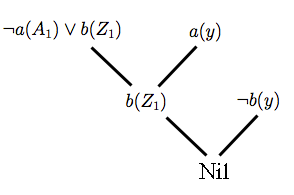
\includegraphics[scale=0.60]{./images/arbolito.png}
\label{modelado}
\end{center}
\end{figure}

\par Aclaración: En el primer nivel se utiliza la sustitución $\{A_1/y\}$ y en el segundo $\{Z_1/y\}$

\section{Demostración 1: $\forall z \  \exists x \  H(z,x)$}

\par Transformación a \textbf{CNF}:

\begin{equation}
F(S_1(y), y)
\end{equation}
\begin{equation}
G(S_2(z),z)
\end{equation}
\begin{equation}
\neg F(u,v) \vee \neg G(v,w) \vee H(u,w)
\end{equation}
\begin{equation}
(\neg H(p,q) \vee F(p, S_3(p,q))) \wedge (\neg H(p,q) \vee G(S_3(p,q)))
\end{equation}

\par Negación de lo que se desea probar llevado a \textbf{CNF}:

\begin{equation}
\neg H(a,x)
\end{equation}

\par Ahora la base del conocimiento estará dada por:


\begin{equation}
F(S_1(y), y)
\end{equation}
\begin{equation}
G(S_2(z),z)
\end{equation}
\begin{equation}
\neg F(u,v) \vee \neg G(v,w) \vee H(u,w)
\end{equation}
\begin{equation}
\neg H(a,x)
\end{equation}
\begin{equation}
\neg H(p,q) \vee F(p, S_3(p,q))
\end{equation}
\begin{equation}
\neg H(p,q) \vee G(S_3(p,q))
\end{equation}

\par Nótese que las funciones $S_1$, $S_2$ y $S_3$ son las introducidas por el proceso de \textit{Skolemización} \\
\par \textbf{Resolución:}\\

\par De \textbf{(11)} y \textbf{(13)} utilizando las substituciones $\{u/p, S_3(p,q)/v\}$ se obtiene
\begin{equation}
\neg G(S_3(p,q), w) \vee \neg H(u,q) \vee H(v,w)
\end{equation}

\par De \textbf{(14)} y \textbf{(15)} utilizando las substituciones $\{q/w\}$ se obtiene

\begin{equation}
\neg H(u,q) \vee H(v,q)
\end{equation}

\par De \textbf{(12)} y \textbf{(16)} utilizando las substituciones $\{a/v, q/x\}$ se obtiene

\begin{equation}
\neg H(u,q)
\end{equation}

\par De \textbf{(11)} y \textbf{(17)} utilizando las substituciones $\{w/q\}$ se obtiene

\begin{equation}
\neg F(u,v) \vee \neg G(v,w)
\end{equation}

\par De \textbf{(9)} y \textbf{(18)} utilizando las substituciones $\{S_1(y)/u, y/v\}$ se obtiene

\begin{equation}
\neg G(y,w)
\end{equation}

\par De \textbf{(12)} y \textbf{(19)} utilizando las substituciones $\{S_2(z)/y, z/w\}$ se obtiene \textbf{NIL}


\section{Demostración 2: $\exists y \  Gato(y) \wedge Mata(curiosidad,y)$}

\par Como primer paso se convierte todo a \textbf{CNF} obteniendo:

\begin{enumerate}
\item $\neg Animal(y)\vee\neg Mata(x,y)\vee\neg Ama(x,z)$
\item $\neg Animal(x)\vee Ama(pedro,x)$
\item $Mata(Pedro,Felix)\vee Mata(curiosidad,Felix)$
\item $Gato(Felix)$
\item $\neg Gato(x)\vee Animal(x)$
\item Negación de lo que se desea probar: $\neg Gato(y)\vee\neg Mata(curiosidad,y)$
\end{enumerate}

\par \textbf{Resolución:} 


\begin{itemize}
\item De $(4)+(5)$ con la sustitución $\{Felix/x\}$ se obtiene

\begin{enumerate}
	\setcounter{enumi}{6}
	\item $Animal(Felix)$
\end{enumerate}

\item De $(4)+(6)$ con la sustitución $\{Felix/y\}$ se obtiene
\begin{enumerate}
	\setcounter{enumi}{7}
	\item $\neg Mata(curiosidad,Felix)$
\end{enumerate}

\item De $(3)+(8)$ se obtiene

\begin{enumerate}
	\setcounter{enumi}{8}
	\item $Mata(Pedro,felix)$
\end{enumerate}

\item De $(7)+(1)$ con la sustitución $\{Felix/y\}$ se obtiene
\begin{enumerate}
	\setcounter{enumi}{9}
	\item $\neg Mata(x,Felix)\vee\neg Ama(x,z)$
\end{enumerate}

\item De $(9)+(10)$ con la sustitución $\{Pedro/x\}$ se obtiene
\begin{enumerate}
	\setcounter{enumi}{10}
	\item $\neg Ama(Pedro,z)$
\end{enumerate}

\item De $(7)+(2)$ con la sustitución $\{Felix/x\}$ se obtiene
\begin{enumerate}
	\setcounter{enumi}{11}
	\item $Ama(pedro,Felix)$
\end{enumerate}
\item De $(11)+(12)$ con la sustitución $\{Felix/z\}$ se obtiene
\begin{enumerate}
	\setcounter{enumi}{12}
	\item \textbf{NIL}
\end{enumerate}
\end{itemize}

\par Como se ha visto en la demostración, se ha logrado demostrar que $\exists y \  Gato(y) \wedge Mata(curiosidad,y)$.

\section{Demostración 3: $\forall x \  Ultimo(cons(2, cons(1, Nil)), x)$}

\par Primero se convierte todo a \textbf{CNF}:

\begin{equation}
Ultimo(cons(x,Nil),x) 
\end{equation}

\begin{equation}
\neg Ultimo(y,z) \vee Ultimo(cons(w,y),z) 
\end{equation}

\begin{equation}
\neg Ultimo(cons(2,cons(1,Nil)),p) 
\end{equation}

\par \ \\

\par \textbf{Resolución:}\\

\par De \textbf{(21)} y \textbf{(22)} utilizando las substituciones $\{z/w, cons(1,Nil)/y, z/p\}$ se obtiene

\begin{equation}
\neg Ultimo(cons(1,Nil),z)
\end{equation}

\par De \textbf{(20)} y \textbf{(23)} utilizando las substituciones $\{1/x, 1/z\}$ se obtiene \textbf{NIL}

\section{Resolución por refutación}

\begin{enumerate}
\item Tony, Mike y John pertenecen al Club Alpino.
\item Cada miembro del Club Alpino es, o esquiador, o alpinista o ambas cosas.
\item A ningún alpinista le gusta que llueva.
\item A todos los esquiadores les gusta que nieve.
\item A Mike no le gusta lo que le gusta a Tony, y le gusta lo que le disgusta a Tony.
\item A Tony le gusta que llueva y que nieve.
\item ¿Quién es un miembro del Club Alpino que es alpinista y no es esquiador?
\end{enumerate}

\par Por cuestiones de practicidad se utiliza el siguiente reemplazo: $T=Tony$, $M=Mike$, $J=John$.\\

\par Definanse las siguientes funciones:

\begin{itemize}
\item Alpino(x): x pertenece al Club Alpino
\item gusta(x,y): al sujeto x le gusta y
\item Esquiador(x): x es esquiador
\item Alpinista(x): x es alpinista
\end{itemize}
\par Luego del pasaje a \textbf{CNF} se obtiene:

\begin{equation}
Alpino(T)
\end{equation}

\begin{equation}
Alpino(M)
\end{equation}

\begin{equation}
Alpino(J)
\end{equation}

\begin{equation}
\neg Alpino(x) \vee Esquiador(x) \vee Alpinista(x)
\end{equation}

\begin{equation}
\neg Alpinista(y) \vee gusta(y,llueve)
\end{equation}

\begin{equation}
\neg Esquiador(z) \vee gusta(z, nieve)
\end{equation}

\begin{equation}
\neg gusta(T,p) \vee \neg gusta(M, p)
\end{equation}

\begin{equation}
gusta(T,p) \vee gusta(M,p)
\end{equation}

\begin{equation}
gusta(T,llueve)
\end{equation}

\begin{equation}
gusta(T, nieve)
\end{equation}

\par \ \\
\par \textbf{Resolución:}\\

\par De \textbf{(30)} y \textbf{(33)} utilizando las substituciones $\{nieve/p\}$ se obtiene

\begin{equation}
\neg gusta(M, nieve)
\end{equation}

\par De \textbf{(29)} y \textbf{(34)} utilizando las substituciones $\{M/z\}$ se obtiene

\begin{equation}
\neg Esquiador(M)
\end{equation}

\par De \textbf{(27)} y \textbf{(35)} utilizando las substituciones $\{M/x\}$ se obtiene

\begin{equation}
\neg Alpino(M) \vee Alpinista(M)
\end{equation}

\par De \textbf{(25)} y \textbf{(36)} se obtiene

\begin{equation}
\neg  Alpinista(M)
\end{equation}


\par De \textbf{(25)} y \textbf{(27)} utilizando las substituciones $\{M/x\}$ se obtiene

\begin{equation}
 Esquiador(M) \vee Alpinista(M)
\end{equation}

\par De \textbf{(35)} y \textbf{(38)} se obtiene

\begin{equation}
Alpinista(M)
\end{equation}

\par De \textbf{(37)} y \textbf{(39)} se obtiene \textbf{NIL}


\end{document}
